\documentclass[a4paper,12pt]{jarticle}
\usepackage[dvipdfmx]{graphicx}
\usepackage{amsmath}
\usepackage{subfigure}
\usepackage{comment}

\setlength{\hoffset}{0cm}
\setlength{\oddsidemargin}{-3mm}
\setlength{\evensidemargin}{-3cm}
\setlength{\marginparsep}{0cm}
\setlength{\marginparwidth}{0cm}
\setlength{\textheight}{24.7cm}
\setlength{\textwidth}{17cm}
\setlength{\topmargin}{-45pt}

\renewcommand{\baselinestretch}{1.6}
\renewcommand{\floatpagefraction}{1}
\renewcommand{\topfraction}{1}
\renewcommand{\bottomfraction}{1}
\renewcommand{\textfraction}{0}
\renewcommand{\labelenumi}{(\arabic{enumi})}
%\renewcommand{\figurename}{Fig.} %図をFig.にする


%図のキャプションからコロン:を消す
\makeatletter
\long\def\@makecaption#1#2{% #1=図表番号、#2=キャプション本文
\sbox\@tempboxa{#1. #2}
\ifdim \wd\@tempboxa >\hsize
#1 #2\par 
\else
\hb@xt@\hsize{\hfil\box\@tempboxa\hfil}
\fi}
\makeatother
% 


\title{電機システム制御特論 \\
Assignment (2016/05/20)\\
}
\author{\vspace{40mm}\\
九州工業大学大学院 \hspace{0mm} 工学府\\
機械知能工学専攻\ \hspace{0mm} 知能制御工学コース \\
\vspace{5mm}\\
所属:\ 西田研究室\\
学籍番号:\ 16344217\\
提出者氏名:\ 津上 \hspace{0mm} 祐典\\\vspace{5mm}\\ }
\date{平成28年\ 5月\ 27日}

\begin{document}

%表紙
\titlepage
\maketitle
\thispagestyle{empty}

\newpage

\thispagestyle{empty}
\tableofcontents

\newpage
\setcounter{page}{1}
%%%%%%%%%%%%%%%%%%%%%%%%
\section{問題}
%%%%%%%%%%%%%%%%%%%%%%%%
%
\begin{figure}[bp]
 \begin{center}
  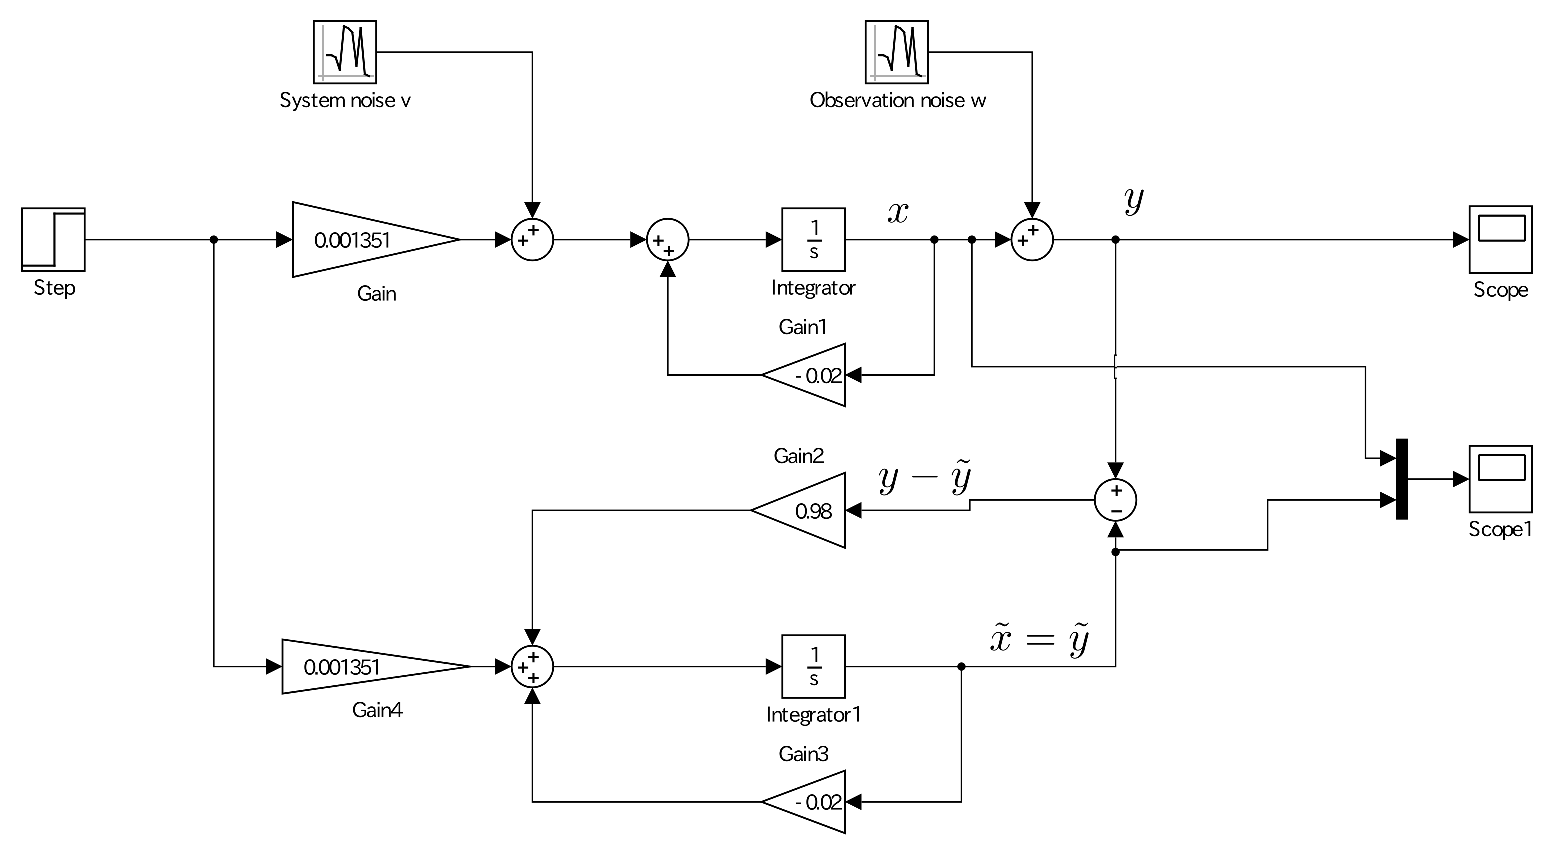
\includegraphics[width = 150mm]{fig/kalmanfilter.eps}
 \end{center}
 \caption{DCモータのブロック線図}
 \label{fig:DC_model}
\end{figure}
%
\begin{figure}[bp]
 \begin{center}
  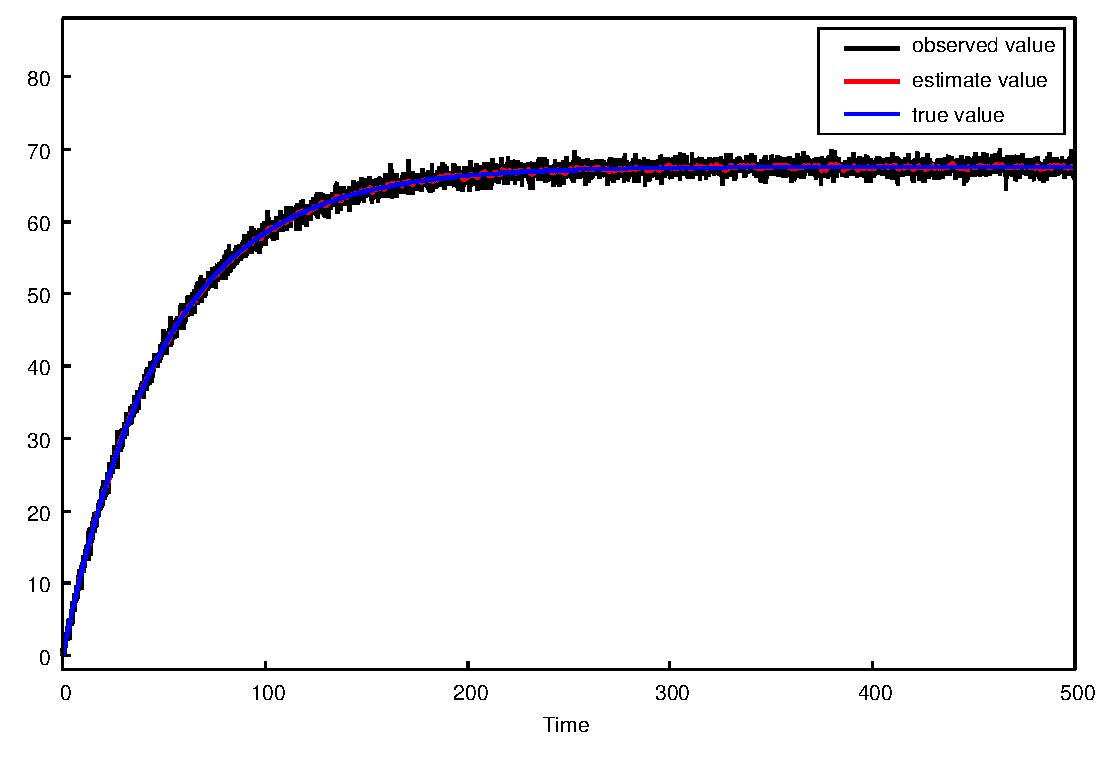
\includegraphics[width = 150mm]{fig/kalmanfilterG.eps}
 \end{center}
 \caption{DCモータのブロック線図}
 \label{fig:DC}
\end{figure}

%
\begin{thebibliography}{99}
\addcontentsline{toc}{section}{参考文献}

 \bibitem{denki} T.Sakamoto,
		 "Lecture Notes of Advanced Electrical Drive Control System", 2016.

 \bibitem{mecha} 坂本哲三, "電気機器の電気力学と制御", 森北出版, 2007.

\end{thebibliography}

\end{document}
